\section{Methodology}
\label{sec:method}

\subsection{System Overview}
The proposed framework operates in two distinct stages (Fig.~\ref{fig:pipeline}). In Stage~1, the denoiser \HSL{} is trained on 8192-sample segments in raw physical millivolt units ($\mathrm{mV}$) to reconstruct clean waveforms without distorting intrinsic signal distributions. In Stage~2, the weights of \HSL{} are frozen, and the model is utilized as an upstream signal purifier for downstream cardiac arrhythmia classification. Extracted 256-sample cardiac beats are normalized and fed into \RRN{}, which fuses morphological features with a 6-dimensional RR timing pathway.

\subsection{Data Model and Physical Preprocessing}
\label{sec:preproc}
Continuous single-lead ECG recordings from the MIT-BIH Arrhythmia Database (sampled at $f_s = 360$\,Hz) are pre-filtered using a 4th-order zero-phase Butterworth bandpass filter ($0.67$--$100$\,Hz):
\begin{equation}
x_f[n] = \mathrm{filtfilt}\big(\mathrm{Butter}_4; [0.67, 100]\,\mathrm{Hz}\big)\{x_{\mathrm{raw}}[n]\}.
\end{equation}
The zero-phase forward-backward filtering attenuates DC drift and ultra-high frequency electrosurgical noise while preserving the temporal phase alignment of R-peaks. Signals are partitioned into segments of length $L = 8192$ samples ($22.75$\,s) with a $50\%$ overlap (hop size $H = 4096$). To remove corrupted flatlines or extreme sensor detachment, segments with energy outside the 5th to 95th percentiles are pruned.

\paragraph*{Physiological Noise Model}
To faithfully emulate clinical environments, realistic noise waveforms from the MIT-BIH Noise Stress Test Database (NSTDB) are superimposed onto clean segments $x_0[n]$:
\begin{equation}
x[n] = x_0[n] + a \sum_{k \in K} \eta_k[n], \quad a = \sqrt{\frac{P_{x_0}}{10^{\mathrm{SNR}/10} P_{\eta}}},
\label{eq:noise_model}
\end{equation}
where $K \subseteq \{\mathrm{bw}, \mathrm{ma}, \mathrm{em}\}$ denotes a subset comprising single, double, or triple noise sources, $P$ represents mean squared power, and $\mathrm{SNR} \in \{-10, -7, -5, -3, 0, 1, 3, 5, 7, 10\}$\,dB controls the contamination severity.

\begin{figure*}[!t]
\centering
\begin{adjustbox}{max width=0.98\textwidth}
\begin{tikzpicture}[
  >=Stealth,
  font=\scriptsize,
  blk/.style={draw, rectangle, rounded corners=2pt, minimum height=7mm, align=center, font=\scriptsize, fill=white, line width=0.6pt},
  io/.style={blk, fill=gray!12, draw=black!70, font=\scriptsize\bfseries},
  stem/.style={blk, fill=teal!10, draw=teal!60!black},
  dwt/.style={blk, fill=teal!22, draw=teal!70!black, font=\scriptsize\bfseries},
  idwt/.style={blk, fill=teal!22, draw=teal!70!black, font=\scriptsize\bfseries},
  enc/.style={blk, fill=blue!10, draw=blue!60!black},
  dec/.style={blk, fill=blue!10, draw=blue!60!black},
  btn/.style={blk, fill=violet!15, draw=violet!70!black, font=\scriptsize\bfseries},
  dg/.style={blk, fill=orange!15, draw=orange!70!black},
  subblk/.style={draw, rectangle, rounded corners=1.5pt, minimum height=4.5mm, minimum width=2.4cm, align=center, font=\tiny, fill=white, line width=0.5pt},
  arr/.style={->, thick},
  plus/.style={circle, draw, fill=orange!20, inner sep=0.5pt, font=\scriptsize\bfseries, minimum size=5mm},
  mul/.style={circle, draw, fill=teal!20, inner sep=0.5pt, font=\scriptsize\bfseries, minimum size=5mm},
  grp/.style={draw=black!60, dashed, rounded corners=3pt, inner sep=2.5mm, font=\scriptsize\bfseries}
]

% ==================== 1. SYMMETRIC U-NET PIPELINE ====================
% Column 0: Input / Output
\node[io] (x_in) at (0, 3.2) {Noisy Input $x[n]$\\($1 \times 8192$, $\mathrm{mV}$)};
\node[plus] (plus) at (0, 0) {$+$};
\node[io] (y_out) at (0, -1.2) {Clean Output $\hat{y}$\\($1 \times 8192$)};

% Column 1: Stem / Out Conv
\node[stem] (stem) at (2.4, 3.2) {Stem Conv\\$1 \to 32, k=3$};
\node[stem] (out_conv) at (2.4, 0) {Out Conv\\$32 \to 1, k=7$\\Correction $\Delta$};

% Column 2: Stage 1 (8192)
\node[enc] (enc1) at (4.8, 3.2) {ResSE Enc 1\\$32 \times 8192$};
\node[dec] (dec1) at (4.8, 0) {ResSE Dec 1\\$32 \times 8192$};

% Column 3: Level 1 DWT / Skip1 / IDWT
\node[dwt] (dwt1) at (7.4, 3.2) {Haar $\DWT_1$\\$\downarrow 2$ ($cA_1, cD_1$)};
\node[dg] (dg1) at (7.4, 1.6) {\textbf{ResSE Skip 1}\\$cD_1 \to S_1$ ($32 \times 4096$)};
\node[idwt] (idwt1) at (7.4, 0) {Haar $\IDWT_1$\\$\uparrow 2$ ($L_1 + S_1$)};

% Column 4: Stage 2 (4096)
\node[enc] (enc2) at (10.0, 3.2) {ResSE Enc 2\\$32 \times 4096$};
\node[dec] (dec2) at (10.0, 0) {ResSE Dec 2\\$32 \times 4096$};

% Column 5: Level 2 DWT / Skip2 / IDWT
\node[dwt] (dwt2) at (12.6, 3.2) {Haar $\DWT_2$\\$\downarrow 2$ ($cA_2, cD_2$)};
\node[dg] (dg2) at (12.6, 1.6) {\textbf{ResSE Skip 2}\\$cD_2 \to S_2$ ($32 \times 2048$)};
\node[idwt] (idwt2) at (12.6, 0) {Haar $\IDWT_2$\\$\uparrow 2$ ($L_2 + S_2$)};

% Column 6: Bottleneck
\node[btn, minimum height=14mm] (btn) at (15.3, 1.6) {ResSE Bottleneck\\($m=1$ block)\\$32 \times 2048$};

% --- Connections: Top Encoder Flow ---
\draw[arr] (x_in) -- (stem);
\draw[arr] (stem) -- (enc1);
\draw[arr] (enc1) -- (dwt1);
\draw[arr] (dwt1) -- node[above, font=\tiny]{$cA_1$} (enc2);
\draw[arr] (enc2) -- (dwt2);
\draw[arr] (dwt2) -- node[above, font=\tiny]{$cA_2$} ++(1.4,0) |- (btn.north);

% --- Connections: Bottleneck to Decoder ---
\draw[arr] (btn.south) |- ++(-1.4,-0.4) -| node[pos=0.25, below, font=\tiny]{$B$} (idwt2.east);

% --- Connections: Bottom Decoder Flow ---
\draw[arr] (idwt2) -- (dec2);
\draw[arr] (dec2) -- (idwt1);
\draw[arr] (idwt1) -- (dec1);
\draw[arr] (dec1) -- (out_conv);
\draw[arr] (out_conv) -- (plus);
\draw[arr] (plus) -- (y_out);

% --- Skip Connections: Straight Vertical Arrows ---
\draw[arr] (dwt1.south) -- node[right, font=\tiny]{$cD_1$} (dg1.north);
\draw[arr] (dg1.south) -- node[right, font=\tiny]{$S_1$} (idwt1.north);

\draw[arr] (dwt2.south) -- node[right, font=\tiny]{$cD_2$} (dg2.north);
\draw[arr] (dg2.south) -- node[right, font=\tiny]{$S_2$} (idwt2.north);

% --- Global Residual Skip ---
\draw[arr] (x_in.south) -- (plus.north);

% Macro Box Container
\begin{scope}[on background layer]
\node[grp, fit=(x_in)(y_out)(btn), label={[font=\footnotesize\bfseries, anchor=south west]north west:\textbf{HaarSymLite Macro U-Net Architecture (75,133 Parameters)}}] (g_macro) {};
\end{scope}

% ==================== 2. DETAILED SUB-BLOCK BREAKOUT (BOTTOM) ====================
% --- Sub-block (a): ResBlock1D ---
\node[subblk] (ise_in) at (2.4, -2.4) {Input $E \in \mathbb{R}^{C \times T}$};
\node[subblk, below=1.2mm of ise_in] (ise_p1) {Conv1D $7\times 1$ ($C \to C$)};
\node[subblk, below=1.2mm of ise_p1] (ise_bn1) {BatchNorm1D + SiLU};
\node[subblk, below=1.2mm of ise_bn1] (ise_dw) {Conv1D $3\times 1$ ($C \to C$) + BN};
\node[plus, below=1.2mm of ise_dw] (ise_plus) {$+$};
\node[subblk, below=1.2mm of ise_plus] (ise_bn2) {SiLU Activation};
\node[subblk, below=1.2mm of ise_bn2, fill=teal!10] (ise_se) {SE1D Channel Attention ($C$)};
\node[subblk, below=1.2mm of ise_se] (ise_out) {Output $E' \in \mathbb{R}^{C \times T}$};

\draw[arr] (ise_in) -- (ise_p1);
\draw[arr] (ise_p1) -- (ise_bn1);
\draw[arr] (ise_bn1) -- (ise_dw);
\draw[arr] (ise_dw) -- (ise_plus);
\draw[arr] (ise_plus) -- (ise_bn2);
\draw[arr] (ise_bn2) -- (ise_se);
\draw[arr] (ise_se) -- (ise_out);
\draw[arr] (ise_in.east) -- ++(2.5mm,0) |- node[pos=0.3, right, font=\tiny]{skip} (ise_plus.east);

\begin{scope}[on background layer]
\node[grp, fit=(ise_in)(ise_out), label={[font=\scriptsize\bfseries, anchor=south west]north west:\textbf{(a) ResSEBlock1D Module}}] (g_ise) {};
\end{scope}

% --- Sub-block (b): Detail Subband Skip ---
\node[subblk] (dg_in) at (7.8, -2.4) {Detail Subband $cD \in \mathbb{R}^{C \times T}$};
\node[subblk, below=1.8mm of dg_in] (dg_dw) {Conv1D $7\times 1$ ($C \to C$) + BN + SiLU};
\node[subblk, below=1.8mm of dg_dw] (dg_bn) {Conv1D $3\times 1$ ($C \to C$) + BN + Skip};
\node[subblk, below=1.8mm of dg_bn, fill=teal!10] (dg_se) {SE1D Channel Attention};
\node[subblk, below=1.8mm of dg_se] (dg_out) {Filtered Detail $S \in \mathbb{R}^{C \times T}$};

\draw[arr] (dg_in) -- (dg_dw);
\draw[arr] (dg_dw) -- (dg_bn);
\draw[arr] (dg_bn) -- (dg_se);
\draw[arr] (dg_se) -- (dg_out);

\begin{scope}[on background layer]
\node[grp, fit=(dg_in)(dg_out), label={[font=\scriptsize\bfseries, anchor=south west]north west:\textbf{(b) Detail Subband Filtering (ResSE)}}] (g_dg) {};
\end{scope}

% --- Sub-block (c): SE1D Module ---
\node[subblk] (se_in) at (13.2, -2.4) {Feature $U \in \mathbb{R}^{C \times T}$};
\node[subblk, below=1.2mm of se_in] (se_gap) {1D Global Avg Pool ($C \times 1$)};
\node[subblk, below=1.2mm of se_gap] (se_fc1) {Linear ($C \to C/4$) + SiLU};
\node[subblk, below=1.2mm of se_fc1] (se_fc2) {Linear ($C/4 \to C$)};
\node[subblk, below=1.2mm of se_fc2] (se_sig) {Sigmoid $\sigma \to$ Weights $a$};
\node[mul, below=1.2mm of se_sig] (se_mul) {$\otimes$};
\node[subblk, below=1.2mm of se_mul] (se_out) {Recalibrated $a \odot U$};

\draw[arr] (se_in) -- (se_gap);
\draw[arr] (se_gap) -- (se_fc1);
\draw[arr] (se_fc1) -- (se_fc2);
\draw[arr] (se_fc2) -- (se_sig);
\draw[arr] (se_sig) -- (se_mul);
\draw[arr] (se_mul) -- (se_out);
\draw[arr] (se_in.east) -- ++(2.5mm,0) |- (se_mul.east);

\begin{scope}[on background layer]
\node[grp, fit=(se_in)(se_out), label={[font=\scriptsize\bfseries, anchor=south west]north west:\textbf{(c) SE1D Channel Attention}}] (g_se) {};
\end{scope}

\end{tikzpicture}
\end{adjustbox}
\caption{Detailed architectural blueprint of the proposed \HSL{} denoiser ($C=32, m=1$, total 75{,}133 parameters). The symmetric U-Net architecture (top) utilizes 2-level Haar DWT to decouple approximation and detail subbands, routing detail bands $cD_1, cD_2$ through dedicated \texttt{ResSEBlock1D} skip connections while the bottleneck processes approximation $cA_2$. All encoder, bottleneck, skip, and decoder stages utilize the unified \texttt{ResSEBlock1D} with SiLU activations. Sub-blocks (bottom) detail: \textbf{(a)} Residual Block with Squeeze-and-Excitation (\texttt{ResSEBlock1D}) with receptive kernels $k_1=7, k_2=3$; \textbf{(b)} High-frequency detail subband residual filtering block; and \textbf{(c)} SE1D channel attention module.}
\label{fig:haarsymlite}
\end{figure*}

\subsection{Stage 1: \HSL{} Architecture}
\label{sec:haarsymlite}
\HSL{} maps a contaminated input segment $x \in \mathbb{R}^{1 \times L}$ to an enhanced clean estimate $\hat{y} \in \mathbb{R}^{1 \times L}$. Fig.~\ref{fig:haarsymlite} illustrates the complete structural diagram.

\subsubsection{Discrete Haar Wavelet Decomposition (DWT/IDWT)}
Rather than applying standard max-pooling or strided convolutions that discard half of the information, \HSL{} incorporates fixed, orthonormal Haar wavelet operators directly within the latent feature pipeline. For a feature channel $u \in \mathbb{R}^T$, the single-level Haar DWT decomposes the sequence into low-frequency approximation $cA$ and high-frequency detail $cD$ ($T/2$ coefficients each):
\begin{align}
cA[n] &= \frac{1}{\sqrt{2}}\big(u[2n] + u[2n+1]\big), \\
cD[n] &= \frac{1}{\sqrt{2}}\big(u[2n+1] - u[2n]\big).
\end{align}
The exact inverse transform ($\IDWT$) perfectly synthesizes the original resolution:
\begin{equation}
u[2n] = \frac{1}{\sqrt{2}}(cA[n] - cD[n]), \quad u[2n+1] = \frac{1}{\sqrt{2}}(cA[n] + cD[n]).
\end{equation}
Because Haar filters are fixed, they introduce zero trainable parameters while halving the temporal dimension at each level ($8192 \to 4096 \to 2048$).

\subsubsection{Unified Residual Block with SE1D Attention (\texttt{ResSEBlock1D})}
To maximize structural simplicity, parameter efficiency, and architectural modularity, all stages across the encoder, bottleneck, skip pathways, and decoder employ an identical, standardized block: \texttt{ResSEBlock1D}. Given an input feature tensor $E \in \mathbb{R}^{C \times T}$, the block comprises two 1D convolutional layers with asymmetrical kernels ($k_1=7, k_2=3$), Batch Normalization, a residual identity addition, and Squeeze-and-Excitation (SE1D) channel attention:
\begin{align}
U_1 &= \phi\Big(\mathrm{BN}\big(\mathrm{Conv}_{7}^{C \to C}(E)\big)\Big), \\
U_2 &= \mathrm{BN}\big(\mathrm{Conv}_{3}^{C \to C}(U_1)\big), \\
U_3 &= \phi(E + U_2), \\
E'  &= \mathrm{SE1D}(U_3),
\end{align}
where $\phi(u) = u \cdot \sigma(u)$ denotes the SiLU activation and $\mathrm{BN}(\cdot)$ denotes batch normalization. The larger primary kernel ($k_1=7$) provides a generous temporal receptive field sufficient to span the rapid depolarization phase of the QRS complex ($80$--$100$\,ms at $360$\,Hz), while the secondary kernel ($k_2=3$) preserves sharp local gradient inflection points at the R-peak apex and S-wave nadir without requiring dilated convolutions.

The SE1D module computes a global channel descriptor via temporal average pooling, followed by a two-layer bottleneck MLP ($C \to C_r \to C$, with $C_r = \max(4, \lfloor C/4 \rfloor) = 8$):
\begin{equation}
z_c = \frac{1}{T}\sum_{t=1}^T U_{3}(c, t), \quad a = \sigma\big(W_2 \phi(W_1 z + b_1) + b_2\big),
\end{equation}
\begin{equation}
\mathrm{SE1D}(U_3)_{c,t} = a_c \cdot U_{3}(c, t).
\end{equation}

\subsubsection{Detail Subband Residual Filtering and Symmetric Decoder}
To ensure that high-frequency electromyographic noise and electrode motion artifacts do not leak into the reconstructed waveform while preserving genuine high-frequency QRS details, detail subbands $cD_1, cD_2$ from each Haar DWT stage are routed through dedicated \texttt{ResSEBlock1D} filtering blocks before merging into the decoder:
\begin{equation}
S_k = \mathrm{ResSEBlock1D}(cD_k), \quad k \in \{1, 2\}.
\end{equation}
In the decoder, the synthesized low-frequency representation $L_k$ and the filtered detail representation $S_k$ are paired as inputs to the $\IDWT$, followed by another \texttt{ResSEBlock1D} stage, restoring full physical resolution without checkerboard interpolation artifacts.

\subsubsection{Global Residual Learning and Mixed Loss Formulation}
The final projection layer outputs a signed waveform correction $\Delta = \mathrm{Conv}^{C \to 1}_7(U_0)$, producing the final estimate $\hat{y} = x + \Delta$. The network is optimized end-to-end via a composite time-domain mixed loss:
\begin{equation}
\mathcal{L}_{\mathrm{mixed}}(\hat{y}, x_0) = \alpha \mathcal{L}_{\mathrm{MSE}}(\hat{y}, x_0) + (1-\alpha) \mathcal{L}_{L_1}(\hat{y}, x_0),
\label{eq:mixed_loss}
\end{equation}
where $\alpha = 0.8$. The $\mathcal{L}_{\mathrm{MSE}}$ term enforces high global signal-to-noise ratio, while the $\mathcal{L}_{L_1}$ term penalizes absolute errors linearly, mitigating the R-peak blunting caused by quadratic MSE penalties on large amplitudes.

\begin{figure*}[!t]
\centering
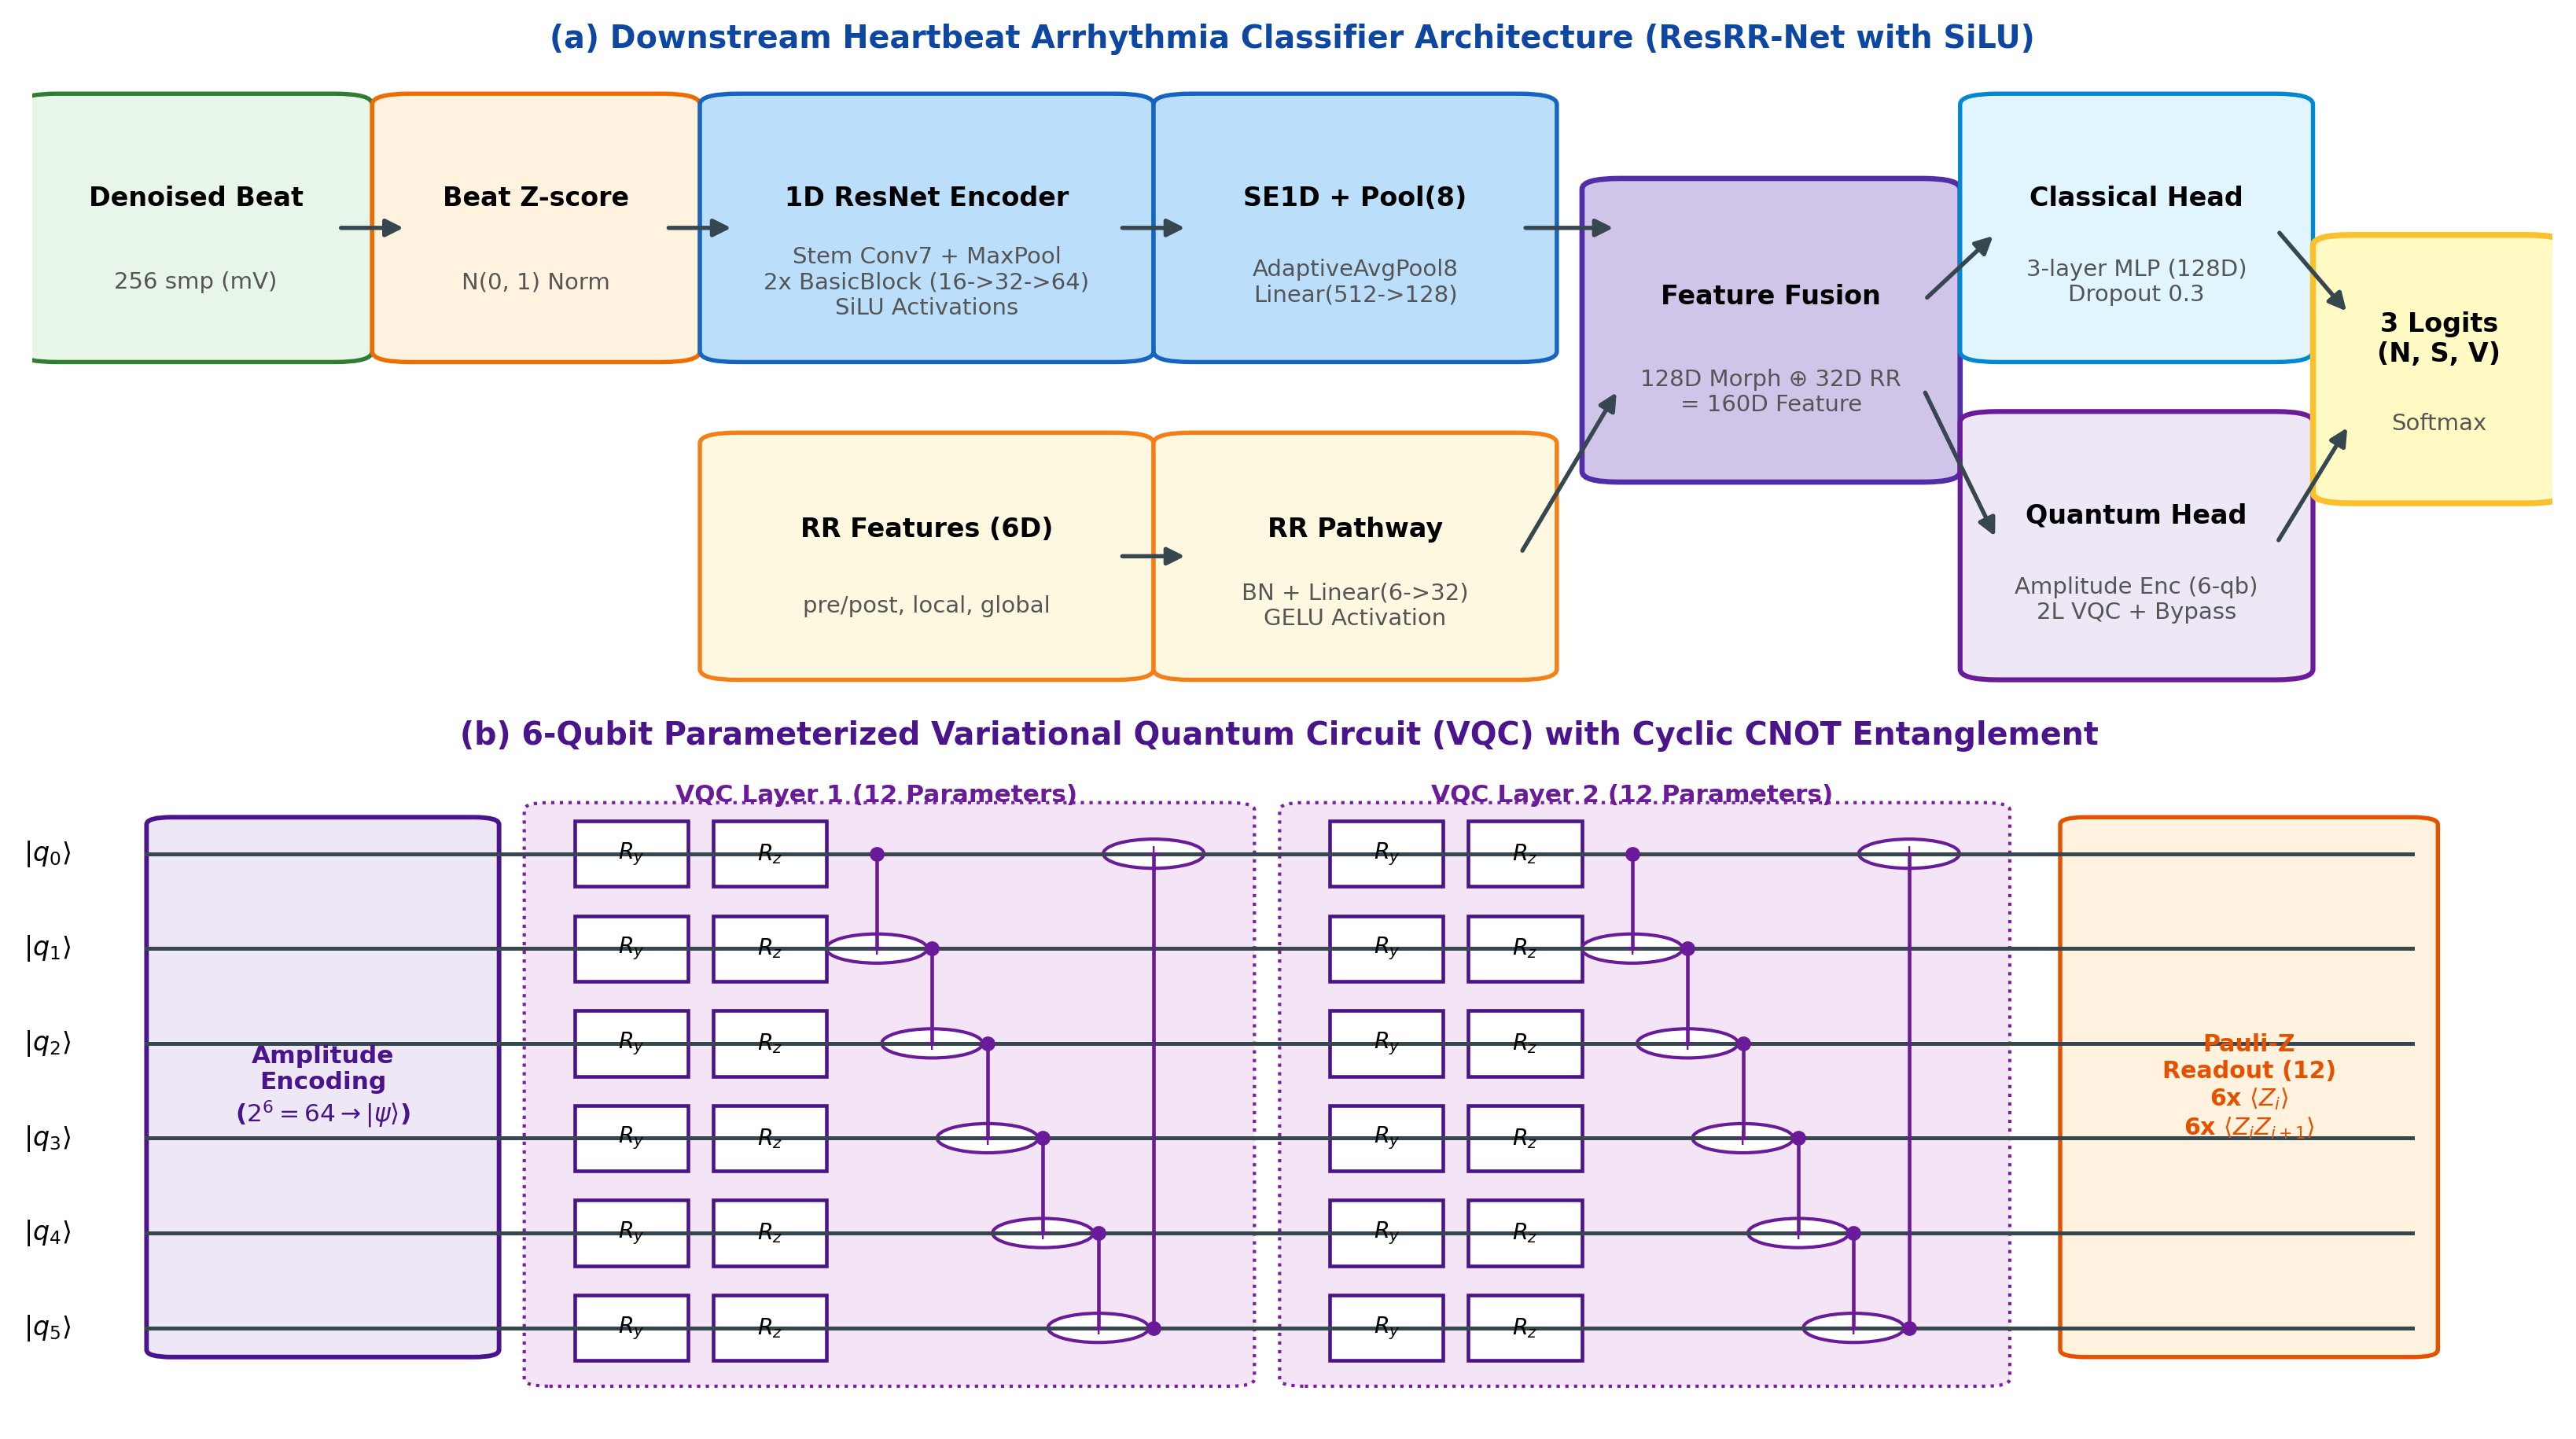
\includegraphics[width=0.98\textwidth]{Fig/fig3_classifier_vqc.png}
\caption{Downstream arrhythmia classification architecture (\RRN). \textbf{(a)} Morphology and RR fusion network: 256-sample denoised beats pass through a 1D ResNet encoder with SE1D attention ($128\text{D}$), concatenated with an independent 6D RR-interval rhythm pathway ($32\text{D}$) to form a $160\text{D}$ feature vector. \textbf{(b)} 6-qubit Parameterized Variational Quantum Circuit (VQC) with amplitude encoding, two variational layers of $R_y(\theta), R_z(\phi)$ single-qubit rotations, cyclic CNOT ring entanglement, Pauli-Z expectation value readout (12 observables), and a parallel classical residual bypass.}
\label{fig:classifier_vqc}
\end{figure*}

\subsection{Stage 2: Beat Classification with \RRN}
\label{sec:classifier}
\subsubsection{Beat Segmentation and Normalization}
Following R-peak locations from reference annotations, individual beats are segmented into windows of $N_b = 256$ samples ($[-90, +165]$ samples around the R-peak, approximately $0.71$\,s), encompassing the full P-QRS-T complex. Denoised beats in physical millivolts are standardized using patient-adaptive Z-score normalization: $\tilde{x} = (x_d - \mu) / (\sigma + 10^{-6})$.

\subsubsection{Independent RR-Interval Pathway}
Because supraventricular ectopic beats (S-class) are morphologically identical to normal beats in single-lead recordings, timing context is decisive. We extract six RR intervals:
\begin{equation}
f_1 = \frac{\mathrm{pre\_RR}}{f_s}, \quad f_2 = \frac{\mathrm{post\_RR}}{f_s}, \quad f_3 = \frac{\mathrm{pre\_RR}}{\overline{RR}_{\mathrm{loc}}},
\end{equation}
\begin{equation}
f_4 = \frac{\mathrm{post\_RR}}{\overline{RR}_{\mathrm{loc}}}, \quad f_5 = \frac{\mathrm{pre\_RR}}{\overline{RR}_{\mathrm{glob}}}, \quad f_6 = \frac{\mathrm{post\_RR}}{\overline{RR}_{\mathrm{glob}}},
\end{equation}
where $\overline{RR}_{\mathrm{loc}}$ is the local moving average over 10 adjacent beats, and $\overline{RR}_{\mathrm{glob}}$ is the global record average. The 6D vector passes through a dedicated pathway ($\mathrm{BatchNorm1D} \to \mathrm{Linear}(6 \to 32) \to \mathrm{GELU}$) and is concatenated with the 128D morphology vector from the 1D ResNet encoder, forming a $160\text{D}$ joint embedding $h \in \mathbb{R}^{160}$ (Fig.~\ref{fig:classifier_vqc}a).

\subsubsection{Dual Interchangeable Classification Heads}
\RRN{} supports two interchangeable heads:
\begin{enumerate}
    \item \textbf{Classical MLP Head:} A 3-layer fully connected network ($160 \to 128 \to 128 \to 3$) with GELU activations and a dropout rate of $0.3$ ($37{,}507$ parameters).
    \item \textbf{Hybrid Quantum Head (VQC):} The 160D vector is compressed to 64D and mapped into the Hilbert state space of 6 qubits ($2^6 = 64$) via amplitude encoding:
    \begin{equation}
    |\psi_{\mathrm{in}}\rangle = \sum_{i=0}^{63} x_i |i\rangle, \quad \sum_{i=0}^{63} |x_i|^2 = 1.
    \end{equation}
    A 2-layer parameterized quantum circuit (Fig.~\ref{fig:classifier_vqc}b) applies single-qubit rotations $R_y(\theta), R_z(\phi)$ followed by a closed cyclic ring of CNOT entangling gates ($q_i \to q_{(i+1)\bmod 6}$), requiring only $2 \times 6 \times 2 = 24$ trainable quantum parameters. Twelve expectation values (6 single Pauli-Z $\langle Z_i \rangle$ and 6 nearest-neighbor correlations $\langle Z_i Z_{i+1} \rangle$) are measured and combined with a parallel 64D classical residual bypass:
    \begin{equation}
    \ell_{\mathrm{qnt}} = W_2 \cdot \mathrm{GELU}\Big(W_1 \big[\langle Z \rangle_{12}; \mathrm{GELU}(W_b h)\big]\Big),
    \end{equation}
    which safeguards against quantum barren plateaus \cite{mcclean2018}. The total hybrid head comprises $30{,}875$ trainable parameters and is simulated using PennyLane \cite{pennylane2018}.
\end{enumerate}

\subsubsection{Imbalance Handling and Soft-Voting Ensemble}
To handle severe class imbalance between normal beats and rare arrhythmias, training samples are drawn using a \texttt{WeightedRandomSampler} with sampling weights $w_c \propto n_c^{-p}$ ($p=0.9$). For each configuration, 5 independent seeds (0 to 4) are trained and aggregated via a Soft-Voting Ensemble:
\begin{equation}
\hat{p}_{\mathrm{ens}}(c \mid x) = \frac{1}{5}\sum_{s=0}^4 \mathrm{softmax}\big(\ell^{(s)}(x)\big)_c.
\end{equation}
